\chapter{Numerical Implementations}
\label{Chap:Numerical}

As mentioned earlier, the simulation of parachute system involves three 
major parts: computational structure dynamics, computational fluid 
dynamics and fluid-structure interaction. 
In this chapter, we discuss the detailed numerical methods for each part. 
The data structures and many functionalities are based on \FronTierp 
library developed for front tracking method \cite{GliGroLi99a,DuFixGli05}.



\section{ODE Solvers}
\label{Sec:ODES}

\subsection{Rigid Body Rotation}
As discussed in the \Sec{RGD}, the governed equations for rigid body 
rotation are \Eqn{eulers_equation2} which is an ODE system. 
We use the fourth-order Runge Kutta method, \Eqn{4th_RK}, to solve for the 
angular velocity $\mathbf{w}$. 
\begin{eqnarray}
\begin{aligned}
u^{n+1} &= u^{n} + h(k_{1} + 2k_{2} + 2k_{3} + k_{4})/6, \\
k_{1} &= \mathscr{L}(t_n, u^{n}), \\
k_{2} &= \mathscr{L}(t_n + h/2, u^{n} + hk_{1}/2), \\
k_{3} &= \mathscr{L}(t_n + h/2, u^{n} + hk_{2}/2), \\
k_{4} &= \mathscr{L}(t_n + h, u^{n} + hk_{3}),
\end{aligned}
\label{eqn:4th_RK}
\end{eqnarray}
where $h$ is the step size and $\mathscr{L}$ is a discretization spatial
operator.

The Euler angles ($\phi$, $\theta$, $\psi$) are visually straightforward.
However, they are difficult to use in numerical computation because of the
involve of trigonometric functions in the rotation matrix 
\Eqn{rotation_matrix1}, which could lead to singularity.
For numerical purpose, we use the four-parameter representation, Euler 
parameters $\mathbf{e} = (e_{0}, e_{1}, e_{2}, e_{3})$, for propagation 
of the rigid bodies, with the constraint \Eqn{Euler_params_constraint}. 
\begin{equation}
e_0^2 + e_1^2 + e_2^2 + e_3^2 = 1
\label{eqn:Euler_params_constraint}
\end{equation}

Euler's rotation theorem states that, in three-dimensional space, any 
displacement of a rigid body such taht a point on the rigid body remain 
fixed, is equivalend to a single rotation about some axis that runs 
through the fixed point. 
This fixed point can be considered as the rotation center. 
The Euler parameters are an interpretation of Euler's rotation theorem, which
is related to an angle of rotation $\alpha$ and a unit vector along the axis 
of rotation $\mathbf{u}$. 
\begin{eqnarray}
\begin{aligned}
e_0 &= \cos(\alpha / 2) \\
\left(
\begin{array}{c}
e_1 \\ e_2 \\ e_3 \\
\end{array}
\right) &= \mathbf{u} \sin(\alpha / 2)
\end{aligned}
\label{eqn:Euler_parameters}
\end{eqnarray}
The initial status means no rotation happens.
Therefore, initially, the Euler parameters are $\mathbf{e} = (1, 0, 0, 0)$.
The relationship between the Euler parameters $\mathbf{e}$ and the angular
velocity $\mathbf{w}$ is given by
\Eqn{euler_parameters_and_angular_velocity}. 
\begin{equation}
\left(
\begin{array}{c}
\dot{e}_0 \\ \dot{e}_1 \\ \dot{e}_2 \\ \dot{e}_3 \\
\end{array}
\right) = \frac{1}{2}
\left(
\begin{array}{ccc}
-e_1 & -e_2 & -e_3 \\
e_0 & e_3 & -e_2 \\
-e_3 & e_0 & e_1 \\
e_2 & -e_1 & e_0 \\
\end{array}
\right)
\left(
\begin{array}{c}
w_1 \\ w_2 \\ w_3 \\
\end{array}
\right)
\label{eqn:euler_parameters_and_angular_velocity}
\end{equation}
As well, fourth-order Runge Kutta method \Eqn{4th_RK} is applied.

Under this circumstance, the rotation matrix $A$ can be written in terms of 
the Euler parameters $\mathbf{e}$ as
\begin{equation}
A =\left(
\begin{array}{ccc}
e_0^2+e_1^2-e_2^2-e_3^2 & 2(e_1e_2+e_0e_3) & 2(e_1e_3-e_0e_2) \\
2(e_1e_2-e_0e_3) & e_0^2-e_1^2+e_2^2-e_3^2 & 2(e_2e_3+e_0e_1) \\
2(e_1e_3+e_0e_2) & 2(e_2e_3-e_0e_1) & e_0^2-e_1^2-e_2^2+e_3^2 \\
\end{array}
\right)
\label{eqn:rotation_matrix}
\end{equation}
The transpose $A^T$ is also the inverse of the rotation matrix $A$. 
$x' = Ax$ represents the rotation process from the world/space coordinates 
system to the body-fixed coordinates system, and $x = A^Tx'$ does the 
opposite process. 
Because the order of rotation in 3 dimensional cases matters, when 
propagating the rigid body from time $t_n$ to $t_{n+1}$, we have the 
following equation.
\begin{equation}
x_{n+1} = A^T_{n+1} A_n x_n
\end{equation}
The subscripts $n$ and $n+1$ are the time step index. This means we always 
first convert to the body-fixed coordinates system before apply the updated 
rotation matrix. 



\subsection{Spring Solver}
\label{Sec:SS}
For the spring-mass model, explicit integration with fourth order 
Runge-Kutta method \Eqn{4th_RK} is adopted to solve the ODE system 
\Eqn{sm_ODEs}.

The explicit scheme requires us to pay attention to the numerical stability 
of the spring solver. 
Based on the previous analysis and numerical verification in 
\cite{LiChernKimLi12, KimLiLi12}, the spring-mass system is a conservative 
system without external forces, and there exists an upper bound for the 
eigenfrequency of the oscillation 
\begin{equation}
w_{max} \leq \sqrt{\frac{2Mk}{m}}, 
\label{eqn:eigenfrequency}
\end{equation}
where $M$ is the maximum number of neighbors that a spring vertex has, $k$ 
is the tensile stiffness and $m$ is the point mass. 
The Delingette's modification adds variation to the spring model, but the 
upper bound is still valid except that the maximum tensile stiffness is used 
in \Eqn{eigenfrequency} instead. 
Therefore, for stability and accuracy purpose, we choose $w_{max}h < 0.1$ for 
simulations.



\section{PDE Solvers}
\label{Sec:PDES}

There have been many techniques to solve the governed equations that describes 
the motion of the fluid. 
For compressible fluid, \Eqn{Euler_eqns_con}, since it is a hyperbolic system, 
we apply the 5th Weighted Essentially Non-Oscillatory (WENO) scheme. 
For incompressible fluid, a pressure correction projection method is used, 
which can achieve second order accuracy. 

\subsection{WENO Scheme}
High-order numerical methods have been widely used to effectively resolve 
complex flow features such as turbulent or vertical flows 
\cite{Ekaterinaris2005192}. 
High-order shock-capturing schemes such as the Essentially Non-Oscillatory 
(ENO) and Weighted ENO (WENO) \cite{Liu1994200,Jiang1996202} schemes not 
only make the computational fluid dynamics (CFD) solvers get rid of 
extremely fine mesh for complex flows, but also perfectly eliminate the 
oscillations near discontinuities. 
WENO scheme is used to reconstruct the spatial derivative term and then the 
hyperbolic system is converted to an ODE system and propagated by 3rd order 
Total Variation Diminishing (TVD) Runge-Kutta method. 

Take one-dimensional Euler equation \Eqn{1d_Euler} for example
\begin{equation}
\mathbf{U}_{t}+\mathbf{F}\left(\mathbf{U}\right)_{x} = 0
\label{eqn:1d_Euler}
\end{equation}
where 
\begin{equation}
\mathbf{U} = 
\left(
\begin{array}{c}
\rho\\ \rho u\\ E
\end{array}
\right),\ 
\mathbf{F}(\mathbf{U}) = 
\left(
\begin{array}{c}
\rho u\\ \rho u^{2}+p\\ (E+p)u
\end{array}
\right)
\end{equation}
\begin{equation}
E = \rho (e+\frac{u^{2}}{2}),\ p = \rho e (\gamma - 1)
\end{equation}
$\rho$, $u$, $P$, $e$ and $\gamma$ denote the density, velocity,
pressure, internal energy per unit mass and ratio of specific heats,
respectively. The Jacobian matrix of the Euler equations is defined as 
\begin{equation}
\mathbf{A} = \frac{\partial \mathbf{F}(\mathbf{U})}{\partial \mathbf{U}}
\end{equation}
The eigenvalues of the Jacobian matrix $A$ are 
\begin{equation}
\lambda_{1} = u-c,\ \lambda_{2}=u,\ \lambda_{3}=u+c
\end{equation}
where $c=\sqrt{\frac{\gamma p}{\rho}}$ is the sound speed, and the
corresponding right eigenvectors are 
\begin{equation}
\mathbf{r}_{1} = 
\left(
\begin{array}{c}
1\\ u-a\\ H-ua
\end{array}
\right),\ 
\mathbf{r}_{2} = 
\left(
\begin{array}{c}
1\\ u\\ \frac{u^{2}}{2}
\end{array}
\right),\ 
\mathbf{r}_{3} = 
\left(
\begin{array}{c}
1\\ u + a\\ H + u a
\end{array}
\right)
\label{eqn:Euler_eigvec}
\end{equation}
where $H$ is the total specific enthalpy, which is related to the
specific enthalpy $h$ and other variables, namely 
\begin{equation}
H = \frac{E + p}{\rho} = \frac{1}{2}u^{2} + h,\ h = e + \frac{P}{\rho}
\end{equation}
We denote the matrix whose columns are eigenvectors in \Eqn{Euler_eigvec} by 
\begin{equation}
\mathbf{R} = \left(\mathbf{r}_{1},\mathbf{r}_{2},\mathbf{r}_{3}\right)
\end{equation}
and denote $\mathbf{L} = \mathbf{R}^{-1}$. The eigenvalue decomposition
of $\mathbf{A}$ is 
\begin{equation}
\mathbf{A} = \mathbf{R \Lambda L}
\end{equation}
where $\mathbf{\Lambda} = diag(u-c,u,u+c)$. Then, \Eqn{1d_Euler} can be 
transformed as 
\begin{equation}
\mathbf{(LU)}_{t} + \Lambda(\mathbf{LU})_{x} = 0
\label{eq:1d_transEuler}
\end{equation}
which consists of three independent one-dimensional hyperbolic equations. 
The advection term in each equation can be reconstructed using WENO scheme 
then solved by advection solver. 

\subsection{Projection Method}
Projection method is an effective way to numerically solve the time-dependent 
incompressible fluid flow problems. 
We apply the pressure-Poisson version of projection method 
\cite{Chorin68, KimMoin85, Brown2001accurate} is adopted to solve the 
Navier-Stokes \Eqn{navierstoke_eqns}. 
\begin{itemize}
\item step 1: Solve for the intermediate velocity $u^*$.
    \begin{eqnarray}
    \begin{aligned}
    \frac{u^* - u^n}{\Delta t} + \frac{1}{\rho} \nabla q &= -[(u \cdot \nabla) u]^{n + \frac{1}{2}} + \frac{\mu}{2\rho} \nabla^2 (u^* + u^n), \\
    B(u^{*}) &= 0, 
    \end{aligned}
    \label{eqn:projection_1}
    \end{eqnarray}
    where $q$ represents an approximation of $p^{n+\frac{1}{2}}$ and 
    $B(u^{*})$ is the boundary condition for $u^{*}$. 
    The term $[(u \cdot \nabla) u]^{n + \frac{1}{2}}$ represents an 
    approximation of the advection term, which is done by WENO scheme. 
    Crank-Nicolson scheme is used to solve this advection-diffusion equation. 
\item step 2: Perform the projection
    \begin{eqnarray}
    \begin{aligned}
    u^* &= u^{n+1} + \Delta t \nabla \phi^{n+1} \\
    \nabla \cdot u^{n+1} &= 0
    \end{aligned}
    \label{eqn:projection_2}
    \end{eqnarray}
    using the boundary conditions consistent with $B(u^{*}) = 0$ and 
    $u^{n+1}|_{\partial \Omega} = u^{n+1}_{b}$. 
    After elimimating $u^{n+1}$, the above two equation becomes a Poisson 
    equation of $\phi$ which is solved by iterative methods. 
\item step 3: Update the pressure.
    \begin{equation}
    p^{n+\frac{1}{2}} = q + \phi^{n+1} - \frac{\mu \Delta t}{2\rho} \nabla^2 \phi^{n+1}.
    \label{eqn:projection_3}
    \end{equation}
    The last term in the above equation gives the second-order accuracy. 
\end{itemize}



\section{Fluid-Structure Interaction}
\label{Sec:FSI}
The interaction between fluid and fabric surface structure is a crucial part 
of the parachute system simulation. 
As mentioned above, the canopy experiences three forces, the gravitational 
force due to the weight of the material, the fluid-generated force due to 
the pressure difference on two sides of the canopy, and the internal spring 
force (both restoring force and friction force). 

\subsection{Force Calculation}
We handle this by the impulse method \cite{KimLiLi12} on the \FronTierp 
platform. 
For each mass point in the spring system, we divide the impulse into three 
components, the gravitational impulse, the fluid impulse and the internal 
impulse due to the spring system, that is, 
\begin{equation}
\mathbf{I}_i^C = \mathbf{I}_{gi}^C + \mathbf{I}_{pi}^C + \mathbf{I}_{si}^C.
\end{equation}
Since no fluid interaction with the string chord is considered in our model, 
the impulse splitting for these mass points is 
\begin{equation}
\mathbf{I}_i^S = \mathbf{I}_{gi}^S + \mathbf{I}_{si}^S.
\end{equation}
The gravitational impulse is straightforward and has the same formula for 
the spring vertex on both the canopy and string chords. 
\begin{equation}
\mathbf{I}_{gi} = \int_{0}^{t} m_{i} \mathbf{g} ds.
\end{equation}
The fluid impulse is 
\begin{equation}
\mathbf{I}_{pi} = \int_{0}^{t} \sigma (p^{-} - p^{+}) \mathbf{n} ds, 
\end{equation}
where $\sigma$ is the mass density of canopy per unity area, $p^{-}$ and 
$p^{+}$ are the pressure on the lower side and upper side of the canopy, 
and $n$ is the unit normal vector pointing from lower to upper side of the 
canopy. 
This follows \cite{Kalro00} for its simplicity. 
A more accurate calculation should also include the velocity shear near the 
canopy surface and stress to the surface. 

For the calculation of the reacting impulse between the canopy and the 
fluid, we apply the immersed boundary method which treats the reaction of 
the canopy as the normal force approximated by the smoothed delta function, 
that is Peskin's delta function, 
\begin{equation}
\mathbf{f}(\mathbf{x}, t) = \int \mathbf{F}(\mathbf{x}, t) \delta(x - \mathbf{X}(s, t)) ds.
\label{eqn:peskin_delta}
\end{equation}
The difference is that we use the impulse of the mass point as a result 
of the superposition of three forces from the spring system, 
\begin{equation}
\mathbf{F}(\mathbf{x}_{i}, t) = d(\mathbf{I}_{g} + \mathbf{I}_{p} + \mathbf{I}_{s}) / dt.
\end{equation}
Numerically, the surface force is the product of the normal component of 
the acceleration and mass density at the canopy surface 
\begin{equation}
\mathbf{F}(s, t) = \rho_{c} (\mathbf{a} \cdot \mathbf{n}) \mathbf{n}, 
\end{equation}
where $\mathbf{n}$ is the unit normal vector on the canopy surface, and 
$\rho_{c}$ is the mass density of canopy per unit area.

\subsection{Local Index Coating}
Our simulation of the parachute system is performed on the \FronTierp 
platform, which uses the front tracking method. 
This method is widely used for tracing the fluid interface in multi-phase 
flow problems, such as the Rayleigh-Taylor instability 
\cite{GliMcBMen86, GliLiMen90}, Richtmyer–Meshkov instability 
\cite{GarGliGro88}, and the jet problems \cite{GliKim04, GliLiOh02}. 
In problems like these, the fluid interface is topologically a manifold, 
the two sides of each surface are the boundaries of two separate domains. 
However, it is not the case in the simulation of parachute system where 
the canopy surface is thinness and forms an open boundary. 
You cannot tell which side of the canopy surface it belongs when a point is 
far away from it. 
But, for points that are sufficiently close to the canopy surface, we can 
still distinguish which side it belongs. 

The reason that we pay attention to this is that the local side information 
of space points that are near the canopy surface contributes to the 
calculation of the pressure difference, and thus the fluid force on the 
canopy. 
The pressure on two sides of the canopy surface is not continuous and it 
should be interpolated using the pressure information on its own side, which 
is realized by locally mesh coating algorithm.
Assign the domain in which the canopy is immersed with index $l$, and the 
local index coating algorithm follows three steps: 
\begin{itemize}
\item For any grid point $P$ with a distance $d \leq h$ away from the canopy, 
where $h$ is the grid spacing, find the nearest point on the canopy surface 
(\FronTierp is well equipped with these geometry functions) $P_{s}$. 
Using the sign of the scalar product $\overline{PP_{s}} \cdot \mathbf{n}_{s}$, 
we can determine the side of the point. 
Reassign domain index to $l-1$ if the point $P$ is on the negative side, 
otherwise reassign the index to $l+1$.
\item Reassign any grid point adjacent to a point indexed $l-1$ to the same; 
reassign any grid point adjacent to a point indexed $l+1$ to the same. 
Repeat this assignment for three sweeps. 
The resulting landscape of the grid index will look like \Fig{local_coating}. 
\item The interpolation of side-sensitive variables will use grid points of 
the same locally coated index.
\end{itemize}
\begin{figure}[!ht]
\centering
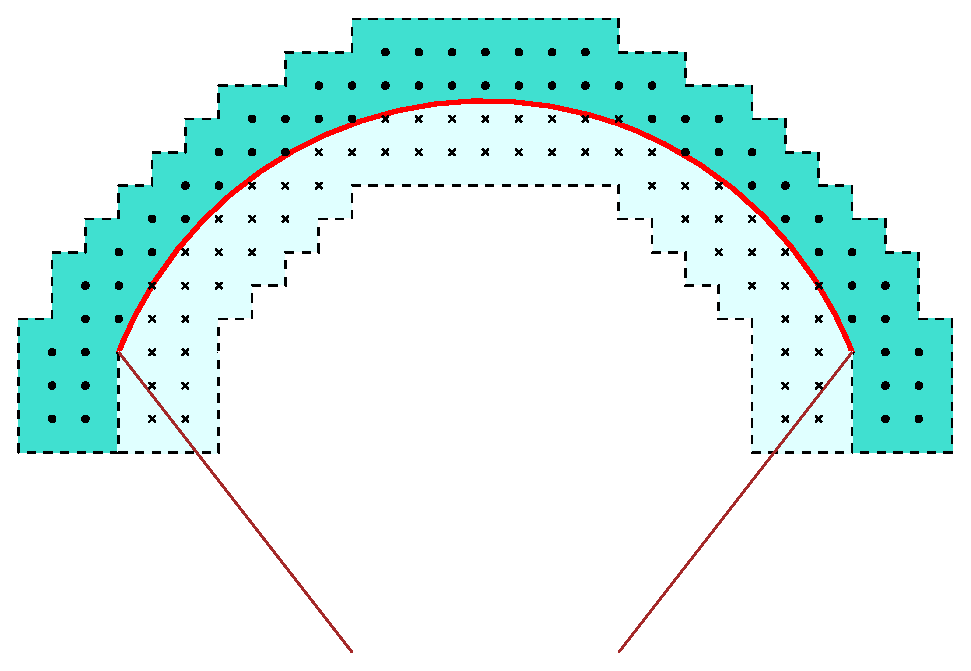
\includegraphics[width=0.7\columnwidth]{figures/local_coating}
\caption{The parachute canopy is an open surface and cannot separate the 
space into sub-domains. But we can still coat different index for mesh 
cells close to the surface using the local geometrical information. The 
light and dark shaded polygons represent the sets of mesh cells on the 
positive and negative sides of the canopy, respectively. An interpolation 
is carried out on vertex of the same color.}
\label{fig:local_coating}
\end{figure}



\section{Collision Features}
\label{Sec:CF}
Collision module for structures is a new feature added to the computational
framework.
With triangulized meshes, the proximity and collision checks can be broken
down into two major cases: a point against a triangle, an edge against
another edge.
For example, when there is collision detected between a pair of triangles,
15 tests need to be done in total.
\begin{itemize}
\item each point of one triangle against the other triangle
\item each edge of one triangle against each edge of the other triangle
\end{itemize}
When strings are taken into account, the comparison pairs can be not only
triangle-triangle, but also edge-edge and edge-triangle, because a string is
represented by a group of connected edges.
Similarly, there is 1 check for a edge-edge pair, and 5 checks for a
edge-triangle pair.

When there are movable rigid bodies involved in collision, we make use of the
impact zone technique which is first proposed in \cite{Provot1997} and further
developed in \cite{Bridson2002collsn}.
This technique was initially proposed to deal with multiple collisions and
maintain collision consistency.
The idea of the impact zone technique is to collect the points in multiple
collisions into separated zones, and treat them as rigid bodies.
Therefore, we can construct each movable rigid body as one independent impact
zone before resolving collisions.
Similar handling as cloth is applied to movable rigid bodies, but we adopted
some differences.
\begin{itemize}
\item The impulse added to each mass point due to collision consists of two
components: inelastic impulse and elastic impulse.
    \begin{itemize}
    \item If the two structures that collid are the same type, i.e. two
    elastic structures or two rigid structures, the inelastic impulse is
    distributed according to the mass
    \begin{equation}
    I_{in, i} = m_{1}m_{2}v_{n} / (m_1 + m_2); 
    \end{equation}
    otherwise, it is distributed evenly
    \begin{equation}
    I_{in,i} = 0.5 m_{i}v_{n}. 
    \end{equation}
    In above, $m_{1}$ and $m_{2}$ are masses and $v_{n}$ is the magnitude of
    relative velocity in the normal direction.
    \item When there is elastic structure(s) involved in the collision,
    the elastic impulse performs like a repulsion due to the elasticity
    \begin{equation}
    I_{el, i} = -min(\Delta t k d, m_{i}(0.1d/\Delta t - v_{n})); 
    \end{equation}
    otherwise, it is the case of two rigid structures
    \begin{equation}
    I_{el, i} = cr I_{in, i}. 
    \end{equation}
    Here, $d$ is the overlap length, $k$ is the string stiffness and $cr$ is
    the restitution coefficient.
    \end{itemize}
\item Whenever an impulse acts on some point on a movable rigid body, it is
spread, via impact zone connection, to all the points on that rigid body.
This is the constraint to maintain the geometric shape of the rigid bodies.
\item The impulse due to cloth-involved collision and that due to rigid
collision are recorded and averaged separately.
Because there will be much more collision detected with cloth, while fewer
between rigid bodies.
\end{itemize}



\newpage
